\newpage
\subsection{GOAL OF LABORATORY WORK}\label{subsec:goal}

Calculate the value of a definite integral with precision $\varepsilon$.

\subsection{TASK DEFINITION}\label{subsec:task_definition}

The Computational Problem:
\begin{enumerate}
    \item Choose precision $\varepsilon$.
    \item Calculate integral with different $A$ and $B$ values from the table.
    \item Calculate execution time of serial program.
    \item {
        Write a parallel program with:
        \begin{itemize}
            \item atomic;
            \item critical sections;
            \item locks;
            \item reduction.
        \end{itemize}
    }
    \item Count speedup with different thread number.
    \item Fill the table (for each point of 4).
\end{enumerate}

\subsection{BRIEF THEORY}\label{subsec:brief_theory}

The \textit{atomic} directive ensures that a specific memory location is updated atomically, rather than exposing it to the possibility of multiple, simultaneous writing threads.

The \textit{critical} directive identifies a construct that restricts execution of the associated structured block to a single thread at a time.

OpenMP 3.0 specifies that \textit{locks} are no longer owned by threads, but by tasks. Once a \textit{lock} is acquired, the current task owns it, and the same task must release it before task completion. The change in \textit{lock} ownership requires extra care when using \textit{locks}.

\textit{Reduction} performs a reduction on the scalar variables that appear in \textit{variable-list}, with the operator \textit{op}. The syntax of the \textit{reduction} clause is as follows: $reduction(op : \text{variable-list })$.
A \textit{reduction} is typically specified for a statement with one of the following forms:
\begin{itemize}
    \item $x = x\text{ }op\text{ }expr$;
    \item $x\text{ }binop = expr$;
    \item $x = expr\text{ }op\text{ }x\text{ (except for subtruction)}$;
    \item $x++$;
    \item $++x$.
\end{itemize}

\subsection{ALGORITHM (METHOD) OF IMPLEMENTATION}\label{subsec:algorithm}

The algorithm for numerical calculation of a certain integral with a given accuracy is shown in the figure~\ref{ris:diag}.

\begin{figure}[H]
    \center
    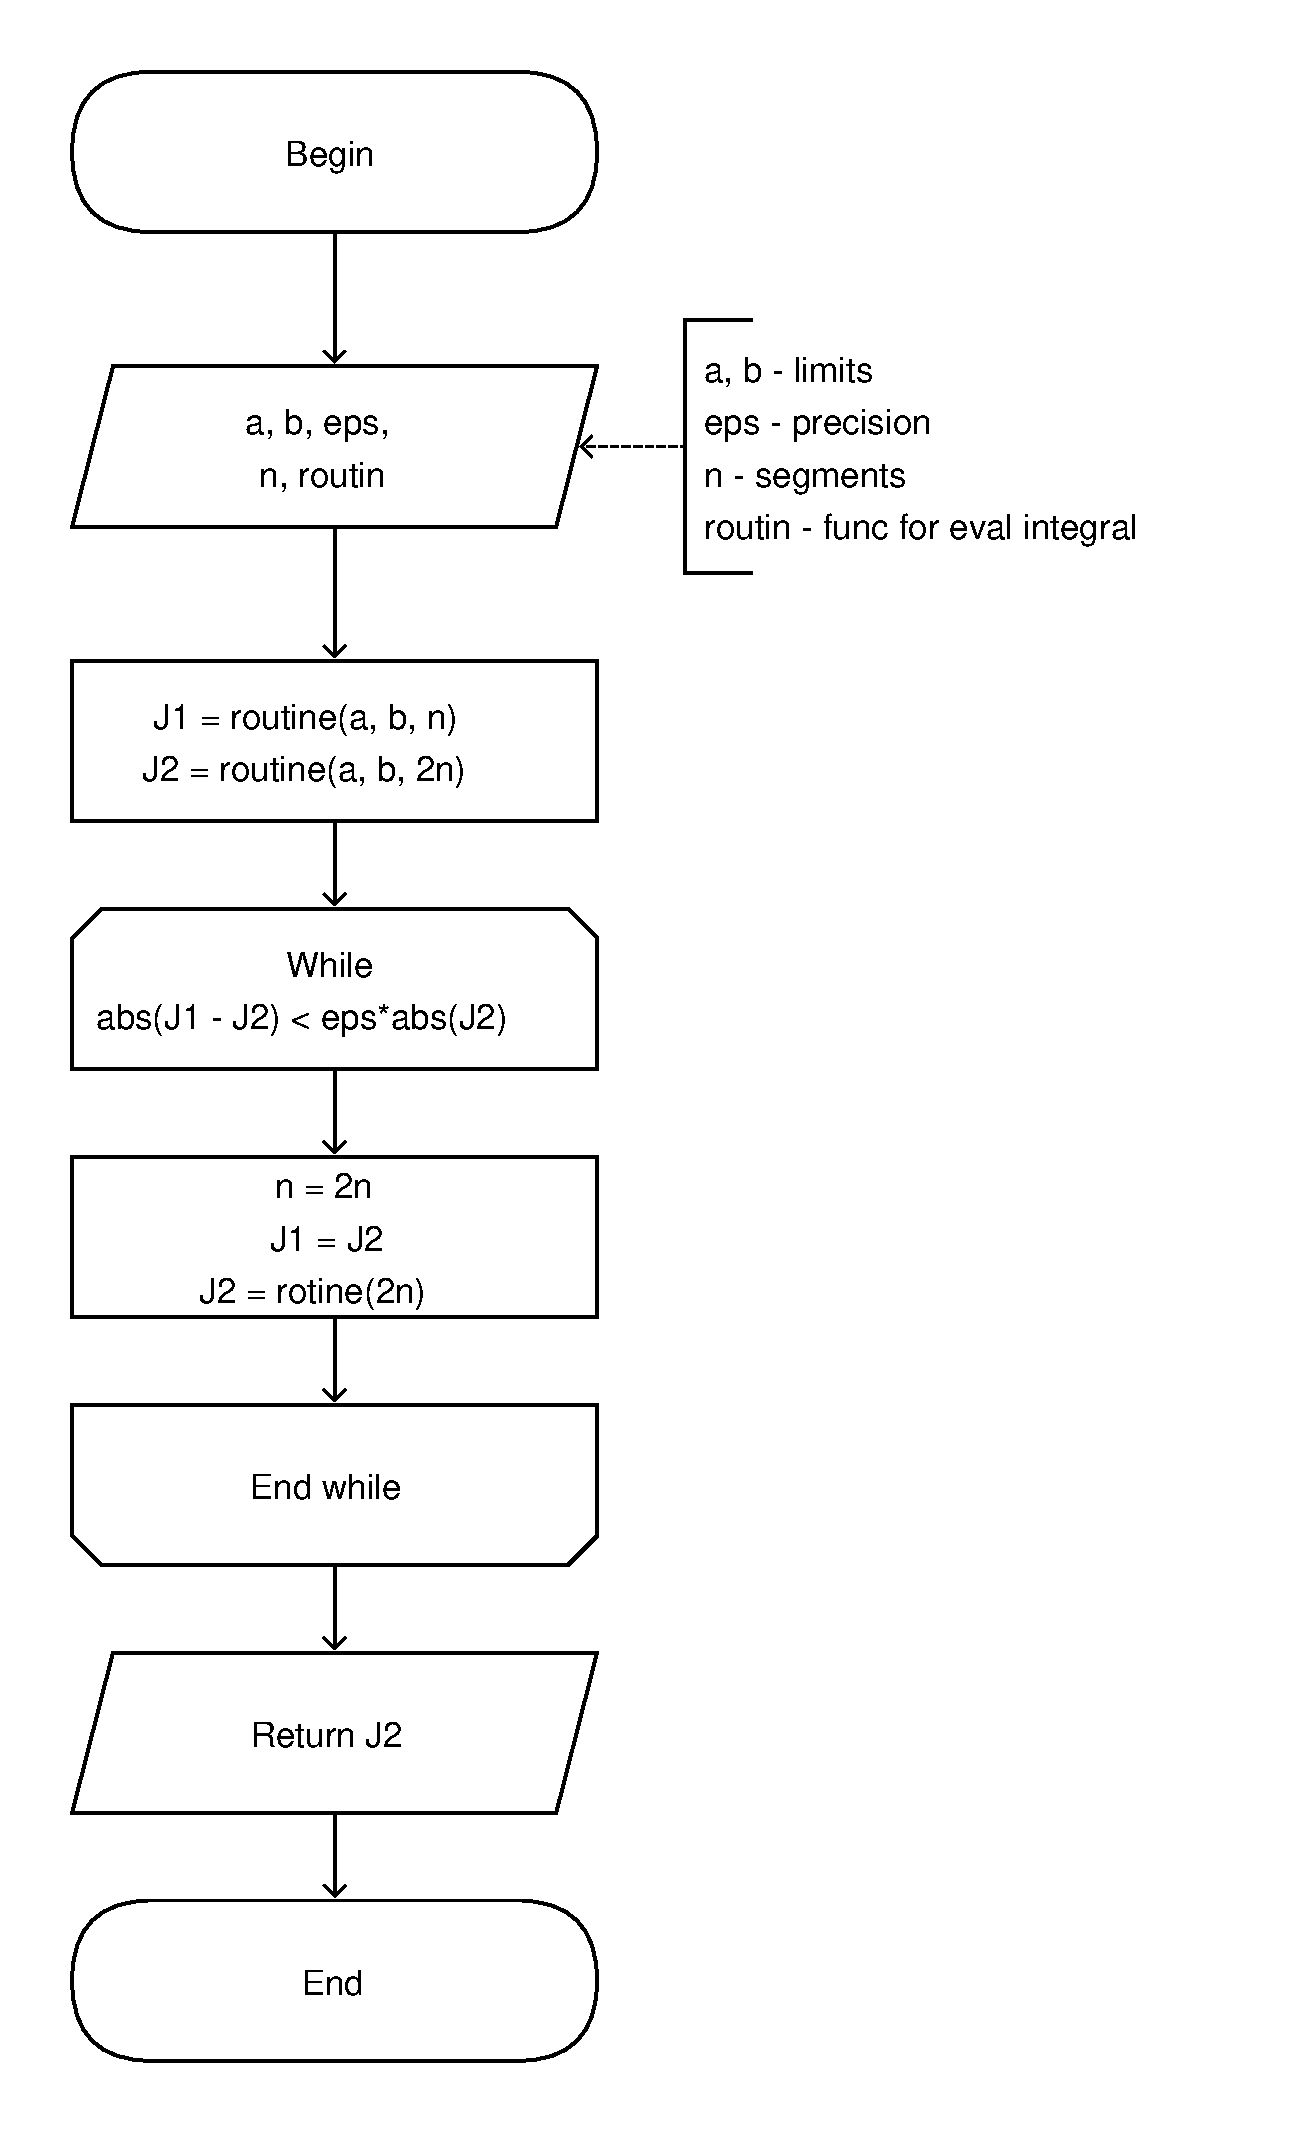
\includegraphics[width=0.8\textwidth]{img/graph.pdf}
    \caption{Diagram of the algorithm}
    \label{ris:diag}
\end{figure}

\subsection{RESULT AND EXPERIMENTS}\label{subsec:result_exp}

The results of measurements for a computer with 4 physical and 8 logical cores and a specified accuracy of $1\mathrm{e}{-6}$ are shown below (Table~\ref{tbl:measure}).

\begin{table}[H]
\caption{Average results of 200 measurements}
\begin{tabular}{ccc|c|c|c|c|c|}
\cline{4-8}
                                            &                                            &         & \multicolumn{5}{c|}{time, ms}                           \\ \hline
\multicolumn{1}{|c|}{a}                     & \multicolumn{1}{c|}{b}                     & threads & serial & atomic & critical\_section & locks & reduction \\ \hline
\multicolumn{1}{|c|}{\multirow{3}{*}{1e-5}} & \multicolumn{1}{c|}{\multirow{3}{*}{1e-4}} & 4       & 0.294  & 0.291  & 0.307             & 0.295 & 0.305     \\ \cline{3-8}
\multicolumn{1}{|c|}{}                      & \multicolumn{1}{c|}{}                      & 8       & 0.315  & 0.309  & 0.303             & 0.305 & 0.310     \\ \cline{3-8}
\multicolumn{1}{|c|}{}                      & \multicolumn{1}{c|}{}                      & 16      & 0.310  & 0.303  & 0.313             & 0.306 & 0.316     \\ \hline
\multicolumn{1}{|c|}{\multirow{3}{*}{1e-4}} & \multicolumn{1}{c|}{\multirow{3}{*}{1e-3}} & 4       & 0.146  & 0.147  & 0.154             & 0.153 & 0.147     \\ \cline{3-8}
\multicolumn{1}{|c|}{}                      & \multicolumn{1}{c|}{}                      & 8       & 0.147  & 0.158  & 0.155             & 0.153 & 0.159     \\ \cline{3-8}
\multicolumn{1}{|c|}{}                      & \multicolumn{1}{c|}{}                      & 16      & 0.155  & 0.167  & 0.158             & 0.164 & 0.156     \\ \hline
\multicolumn{1}{|c|}{\multirow{3}{*}{1e-3}} & \multicolumn{1}{c|}{\multirow{3}{*}{1e-2}} & 4       & 0.079  & 0.073  & 0.073             & 0.072 & 0.072     \\ \cline{3-8}
\multicolumn{1}{|c|}{}                      & \multicolumn{1}{c|}{}                      & 8       & 0.076  & 0.073  & 0.074             & 0.075 & 0.076     \\ \cline{3-8}
\multicolumn{1}{|c|}{}                      & \multicolumn{1}{c|}{}                      & 16      & 0.076  & 0.078  & 0.077             & 0.084 & 0.076     \\ \hline
\multicolumn{1}{|c|}{\multirow{3}{*}{0.01}} & \multicolumn{1}{c|}{\multirow{3}{*}{0.1}}  & 4       & 0.038  & 0.037  & 0.036             & 0.037 & 0.040     \\ \cline{3-8}
\multicolumn{1}{|c|}{}                      & \multicolumn{1}{c|}{}                      & 8       & 0.037  & 0.037  & 0.037             & 0.040 & 0.037     \\ \cline{3-8}
\multicolumn{1}{|c|}{}                      & \multicolumn{1}{c|}{}                      & 16      & 0.037  & 0.036  & 0.037             & 0.037 & 0.037     \\ \hline
\multicolumn{1}{|c|}{\multirow{3}{*}{0.1}}  & \multicolumn{1}{c|}{\multirow{3}{*}{1}}    & 4       & 0.035  & 0.035  & 0.035             & 0.037 & 0.035     \\ \cline{3-8}
\multicolumn{1}{|c|}{}                      & \multicolumn{1}{c|}{}                      & 8       & 0.035  & 0.035  & 0.037             & 0.035 & 0.036     \\ \cline{3-8}
\multicolumn{1}{|c|}{}                      & \multicolumn{1}{c|}{}                      & 16      & 0.035  & 0.035  & 0.035             & 0.039 & 0.037     \\ \hline
\multicolumn{1}{|c|}{\multirow{3}{*}{1}}    & \multicolumn{1}{c|}{\multirow{3}{*}{10}}   & 4       & 0.003  & 0.003  & 0.003             & 0.003 & 0.003     \\ \cline{3-8}
\multicolumn{1}{|c|}{}                      & \multicolumn{1}{c|}{}                      & 8       & 0.003  & 0.003  & 0.003             & 0.004 & 0.003     \\ \cline{3-8}
\multicolumn{1}{|c|}{}                      & \multicolumn{1}{c|}{}                      & 16      & 0.003  & 0.003  & 0.003             & 0.003 & 0.003     \\ \hline
\multicolumn{1}{|c|}{\multirow{3}{*}{10}}   & \multicolumn{1}{c|}{\multirow{3}{*}{100}}  & 4       & 0.003  & 0.003  & 0.003             & 0.003 & 0.003     \\ \cline{3-8}
\multicolumn{1}{|c|}{}                      & \multicolumn{1}{c|}{}                      & 8       & 0.003  & 0.003  & 0.003             & 0.003 & 0.003     \\ \cline{3-8}
\multicolumn{1}{|c|}{}                      & \multicolumn{1}{c|}{}                      & 16      & 0.003  & 0.003  & 0.003             & 0.003 & 0.003     \\ \hline
\end{tabular}
\label{tbl:measure}
\end{table}

In theory, the best result should be given by the "reduction" operation on 8 threads, but due to the simplicity of the task and the CPU load of background tasks, the results were ambiguous.

Based on the description of other methods for providing exclusive access, threads should be blocked for addition operations when calculating the amount. Thus, this section is critical and the execution time should increase.

It is also worth noting that with 16 threads, pseudo-parallelism begins, when one thread takes resources from another.

\subsection{CONCLUSION}\label{subsec:conclusion}

You have to carefully select the appropriate blocking methods for each task. Depending on the computer, the optimal number of threads may vary.

\subsection{APPENDIX}\label{subsec:appendix}

The source code is located \href{https://github.com/vanSultan/parallel_algorithm/tree/lab_01/lab_01}{here}: \url{https://github.com/vanSultan/parallel_algorithm/tree/lab_01/lab_01}.
